%!TEX root = ../../ClassicThesis.tex
%-------------------------------------------------------------------------------
\section{Introduction}
%-------------------------------------------------------------------------------

%-------------------------------------------------------------------------------
\section{Results}
%-------------------------------------------------------------------------------

\subsection{Coherence}

Spectral coherence is the Fourier analogue of linear correlation.
We computed the coherence between the \SIrange{31.3}{97.8}{Hz} range for pairs of depths.
Coherence between channels was computed using the Welch method using \SI{256}{\milli\second} windows with \SI{50}{\percent} overlap.

\begin{figure}[htb]
    \centering
    \hspace*{\fill}
    \subfloat[\ac{LFP}\label{fig:lam_coher_lfp}]{
        \includegraphics[scale=.5]{coherence/coherence-avg_paper_Cln.png}
}
    \hspace*{\fill}\hspace{.2cm}\hspace*{\fill}
    \subfloat[\ac{CSD}\label{fig:lam_coher_csd}]{
        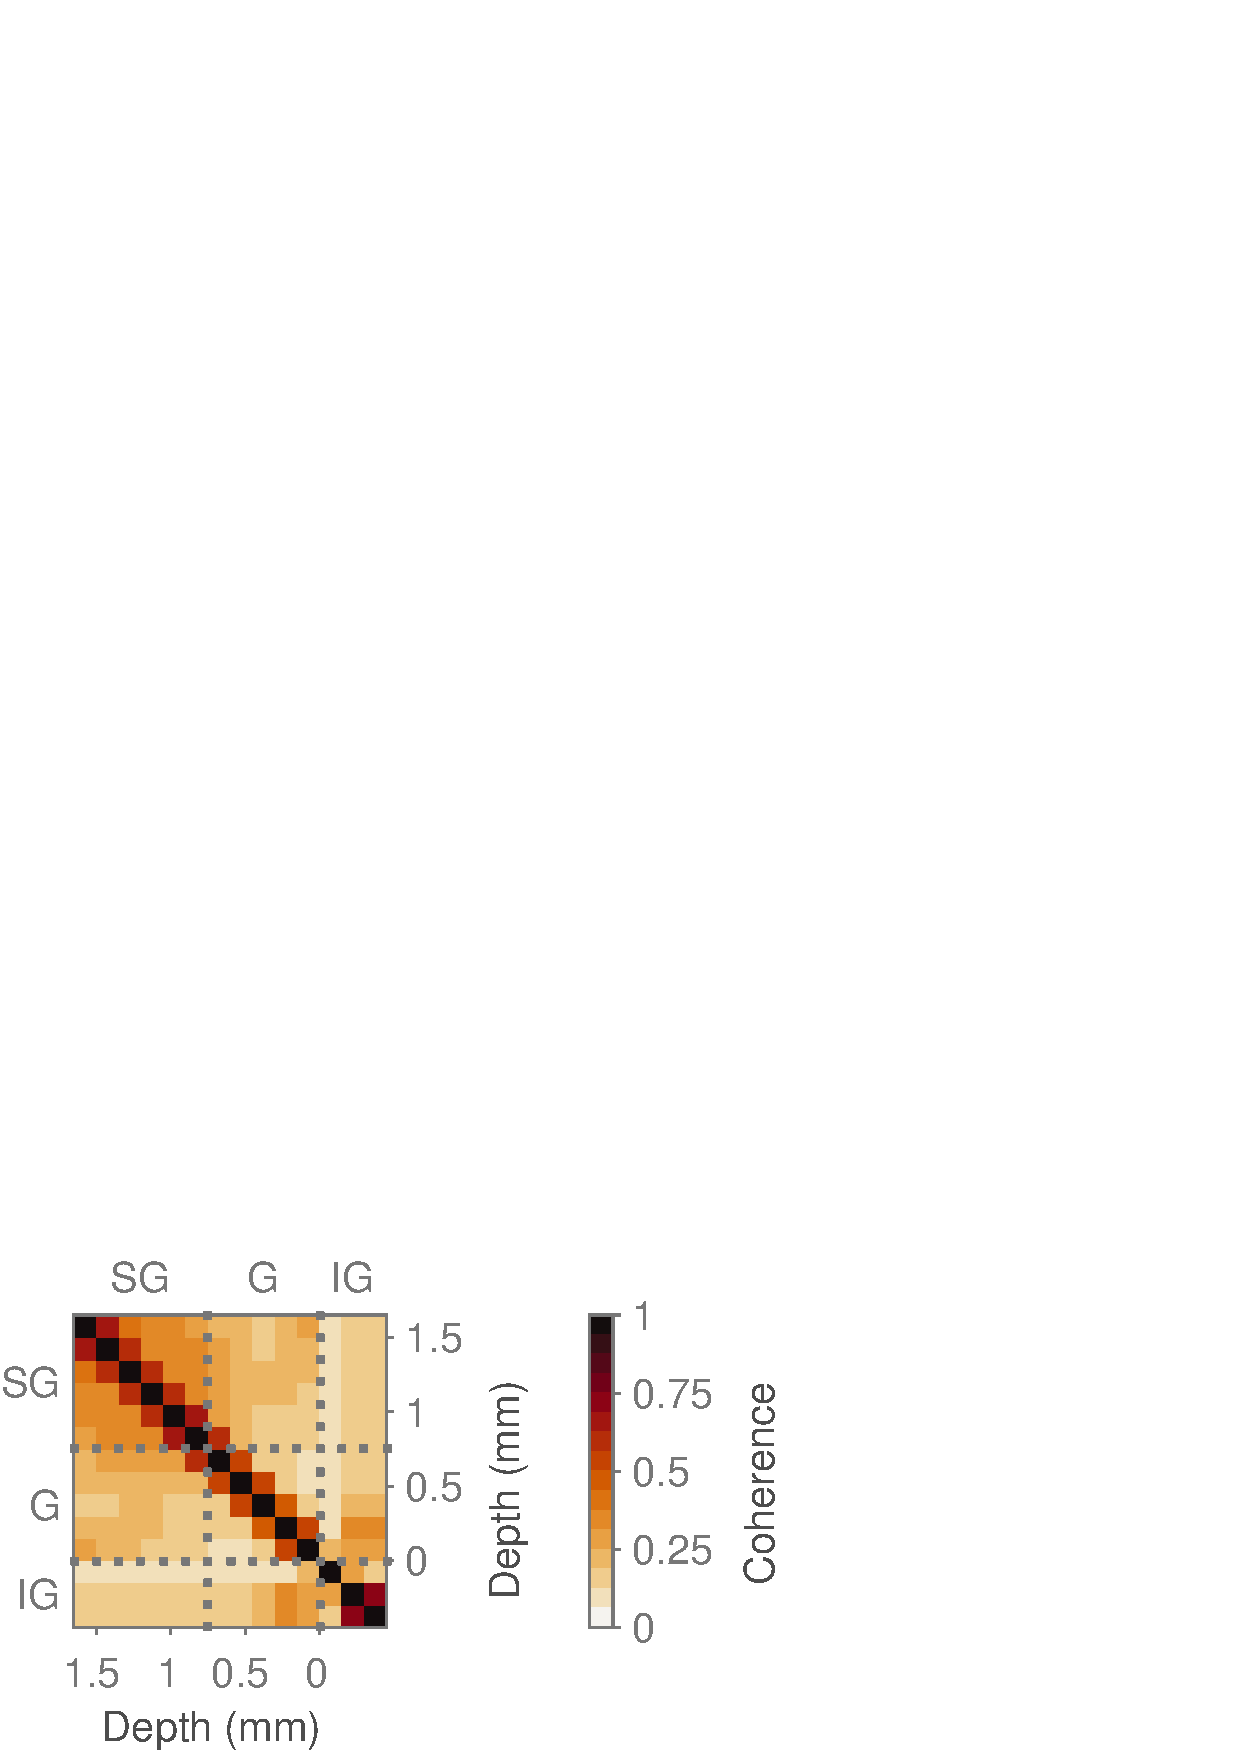
\includegraphics[scale=.5]{coherence/coherence-avg_paper_Csd.png}
}
    \hspace*{\fill}
    \caption{Coherence \SIrange{31.3}{97.8}{Hz}
\protect\subref{fig:lam_coher_lfp}:~\ac{LFP}.
\protect\subref{fig:lam_coher_csd}:~\ac{CSD}.
}
\label{fig:lam_coher}
\end{figure}

The results show the same compartmentalisation as we observed for the information redundancy in the high frequency range, namely that \ac{G} and \ac{SG} are more correlated in the higher frequency ranges than they are with \ac{IG}.

The results for the coherence of the \ac{LFP} (Fig.~\ref{fig:lam_coher_lfp}) show more coherence than the \ac{CSD} (Fig.~\ref{fig:lam_coher_csd}).
This is to be expected since the \ac{CSD} is a better representation of the current sources within the cortex, whose broad extent induces voltage differences (and hence \ac{LFP}) across a larger amount of cortex.

Our results are in agreement with the observations of \citet[Figure 5B]{Maier2010}.

%-------------------------------------------------------------------------------
\subsection{Latency}

\begin{figure}[htb]
    \centering
    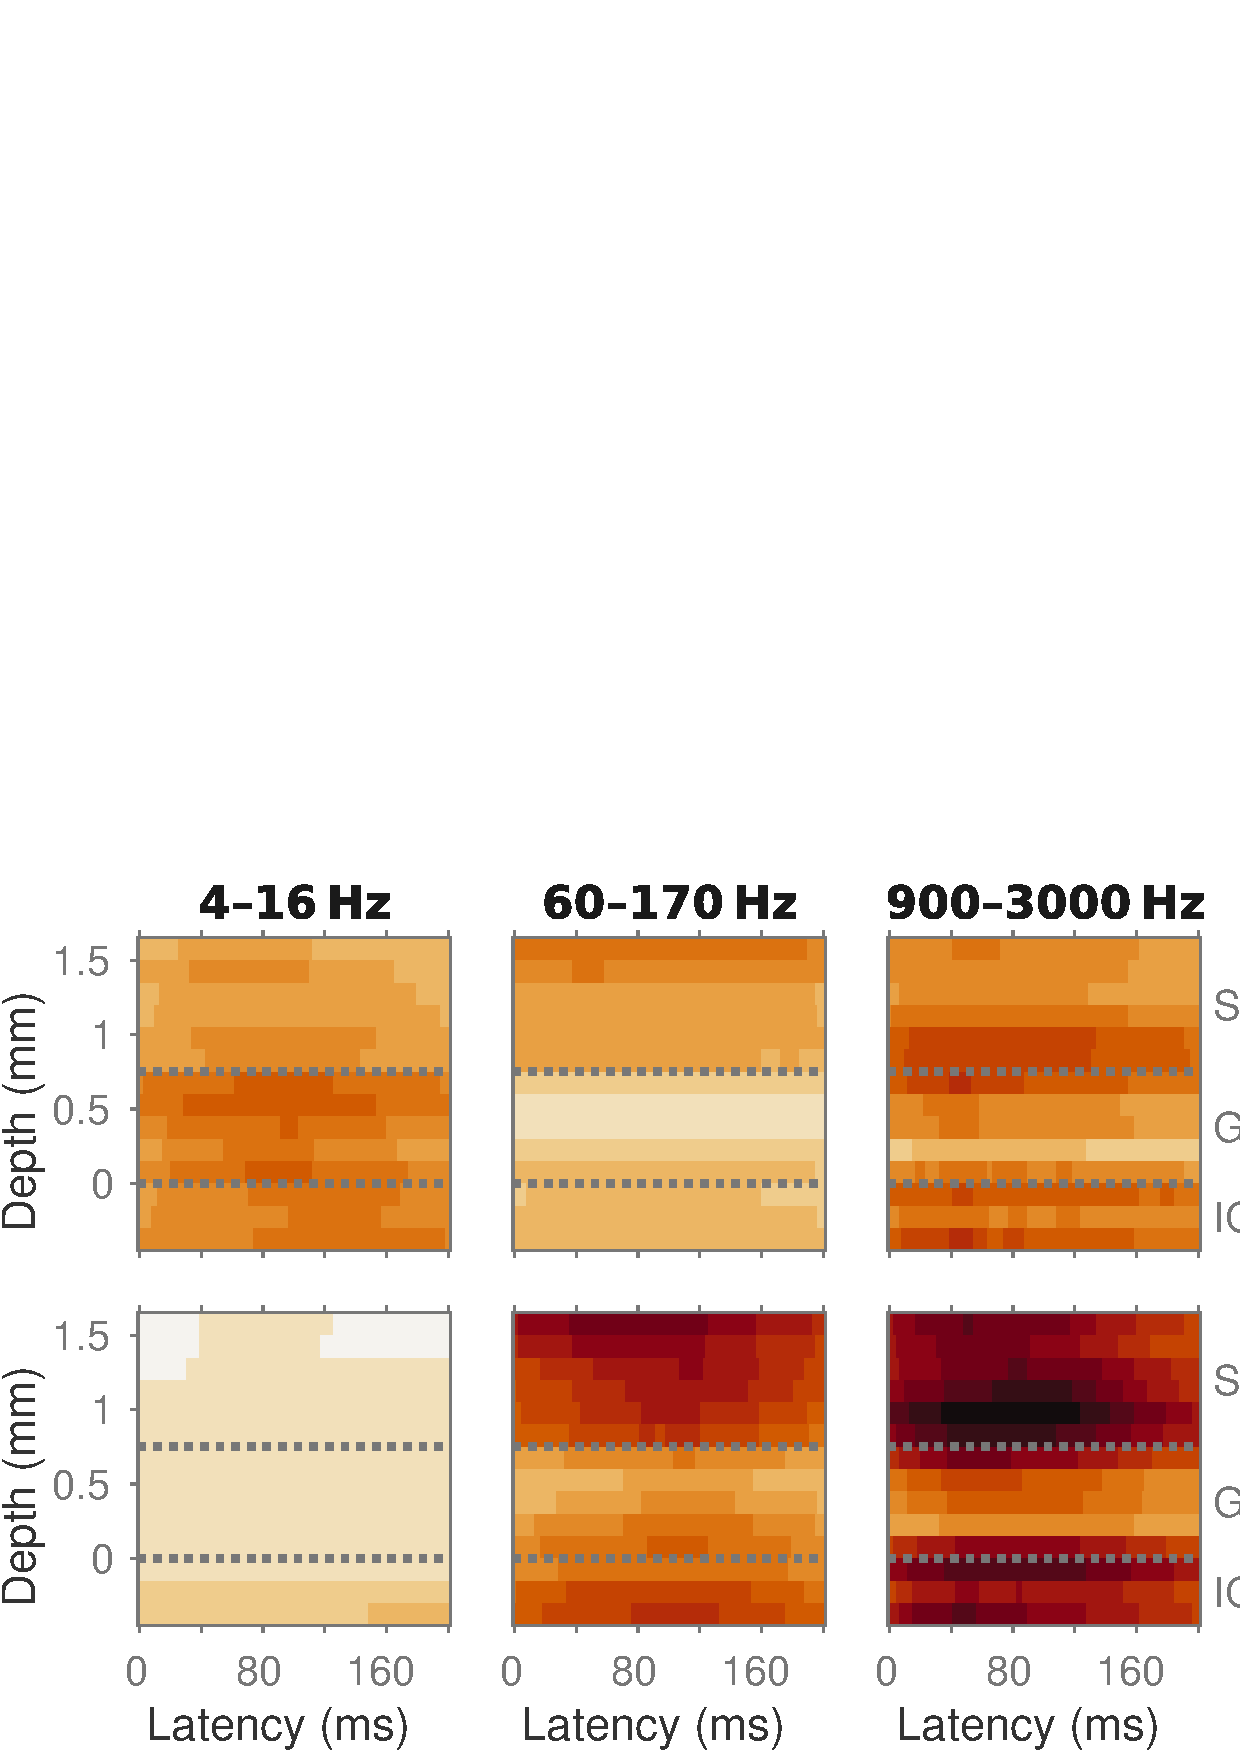
\includegraphics[scale=.5]{lag/lag-heatmap-avg.png}
    \caption{
Information between stimulus and response as a function of the delay between them.
Information contained in \SIrange{4}{16}{Hz} (left), \SIrange{60}{170}{Hz} (middle) and \SIrange{900}{3000}{Hz} (right) power about luminance changes of \SI{<0.3}{cpd} (upper) and \SI{>1.0}{cpd} spatial frequencies.
}
\label{fig:lam_lag_hm}
\end{figure}


\begin{figure}[htb]
    \centering
    \hspace*{\fill}
    \subfloat[\label{fig:lam_lag_cut}]{
        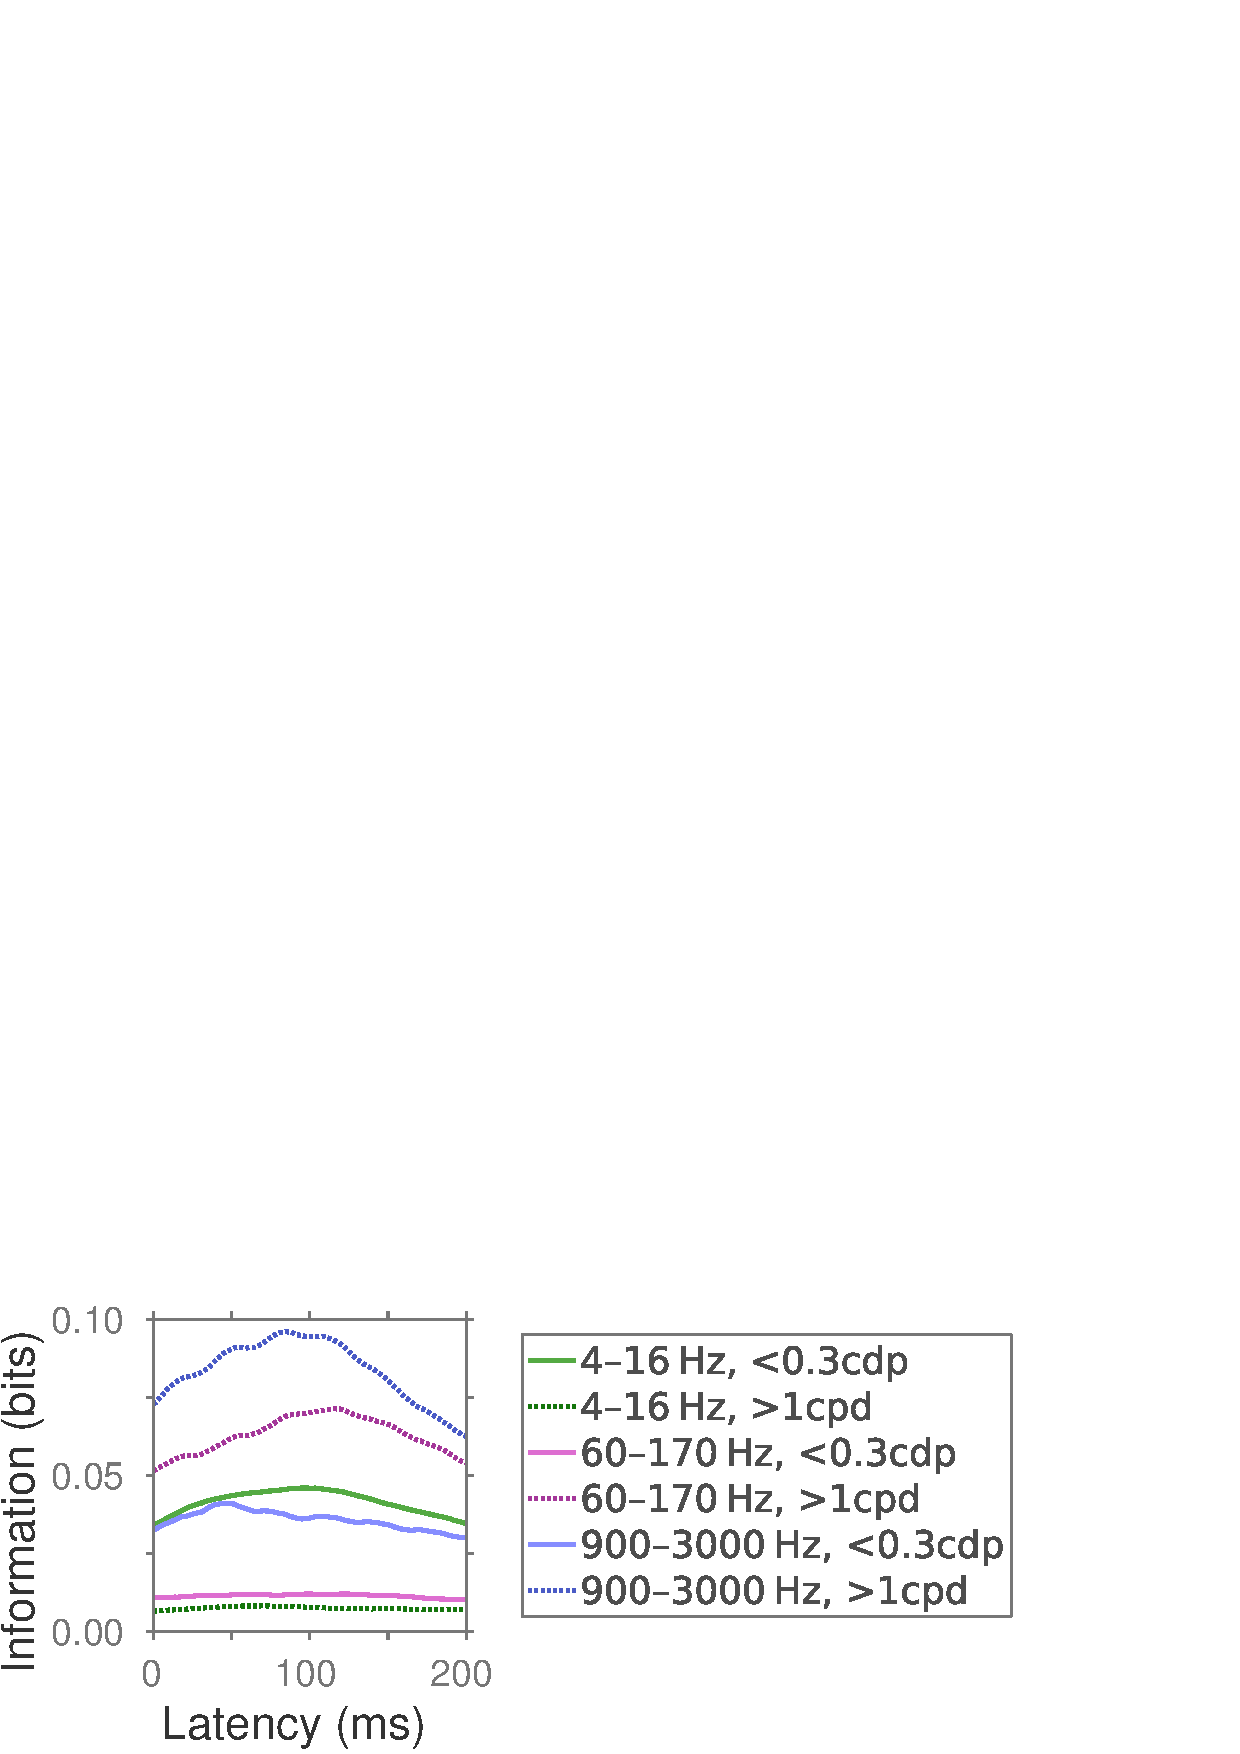
\includegraphics[scale=.5]{lag/lag-line-cut-avg.png}
}
    \hspace*{\fill}\hspace{.2cm}\hspace*{\fill}
    \subfloat[\label{fig:lam_lag_latency}]{
        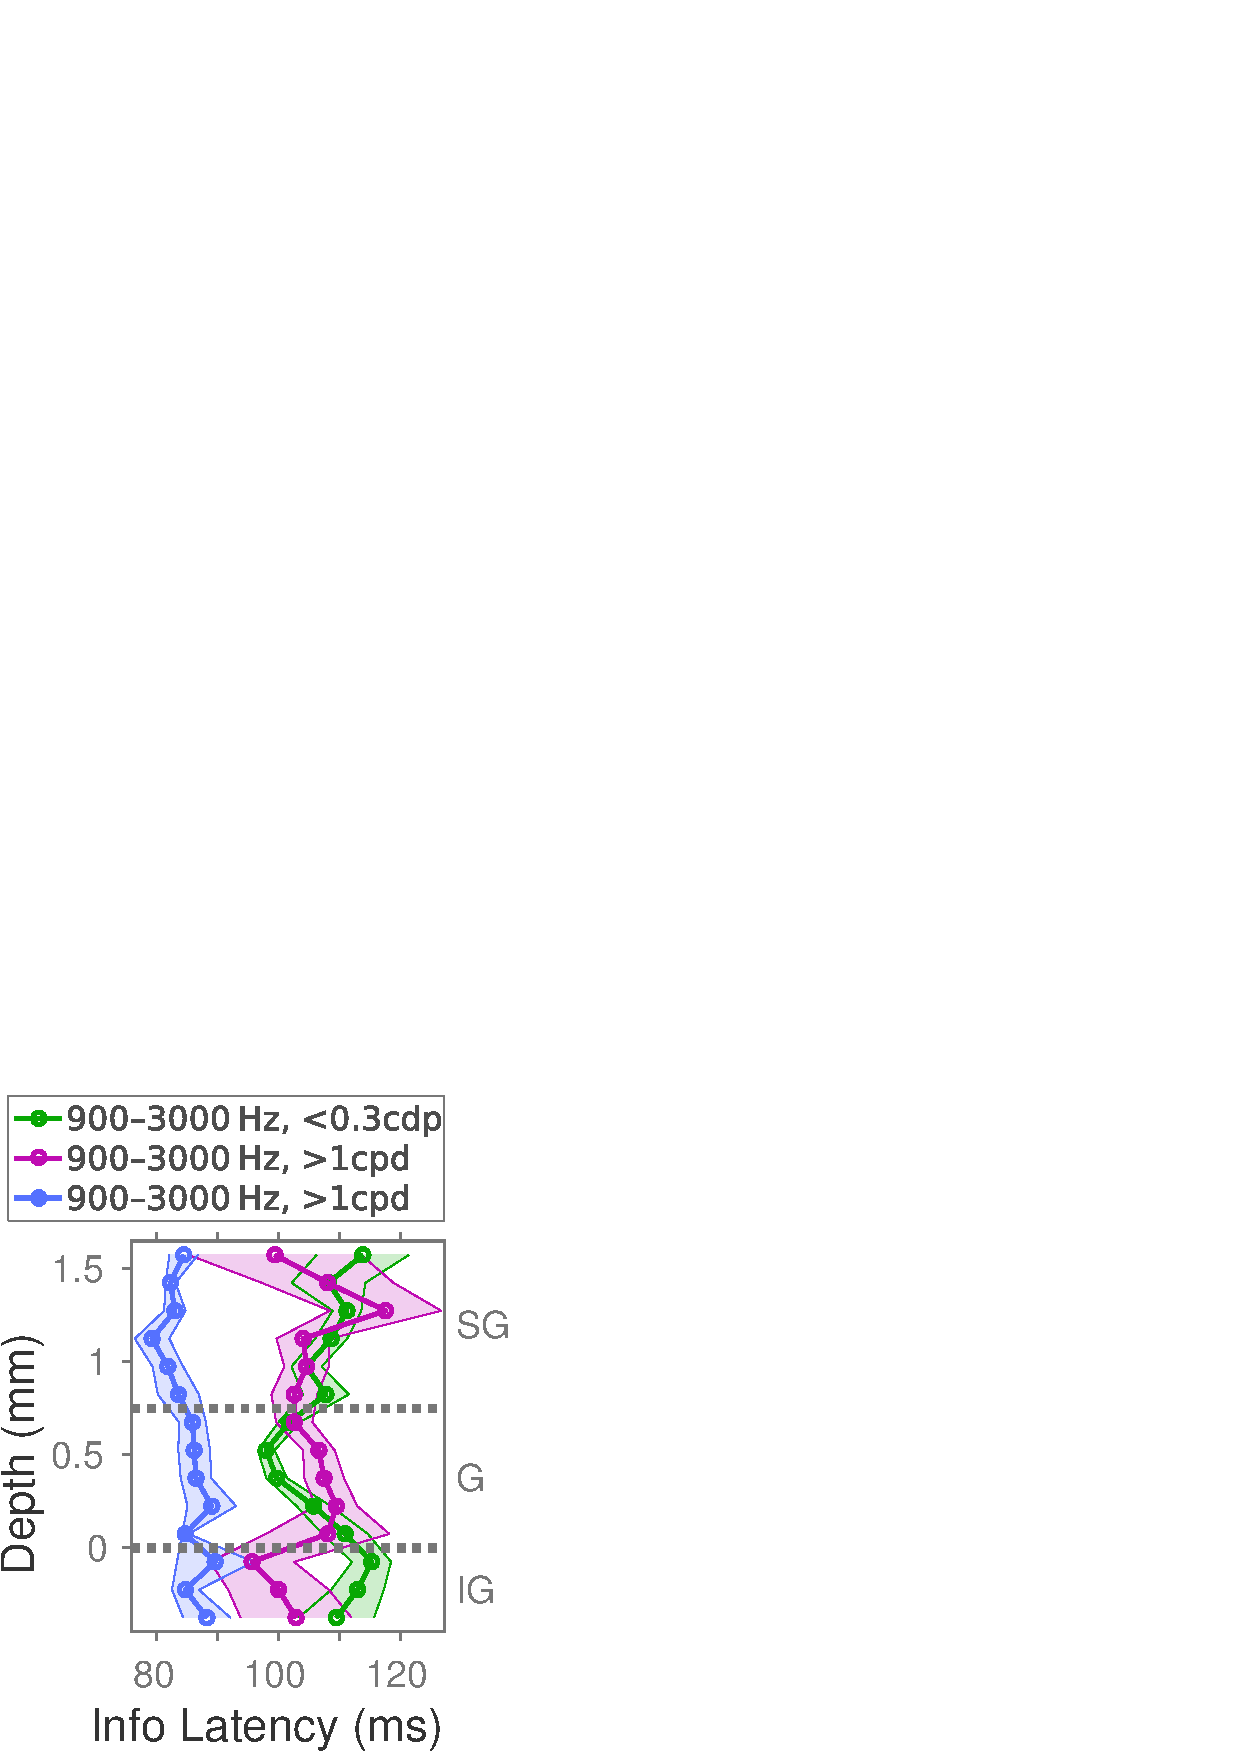
\includegraphics[scale=.5]{lag/rellagpeak3_mean-of-eachband_avg.png}
}
    \hspace*{\fill}
    \caption{
}
\label{fig:lam_lag}
\end{figure}


\begin{figure}[htb]
    \centering
    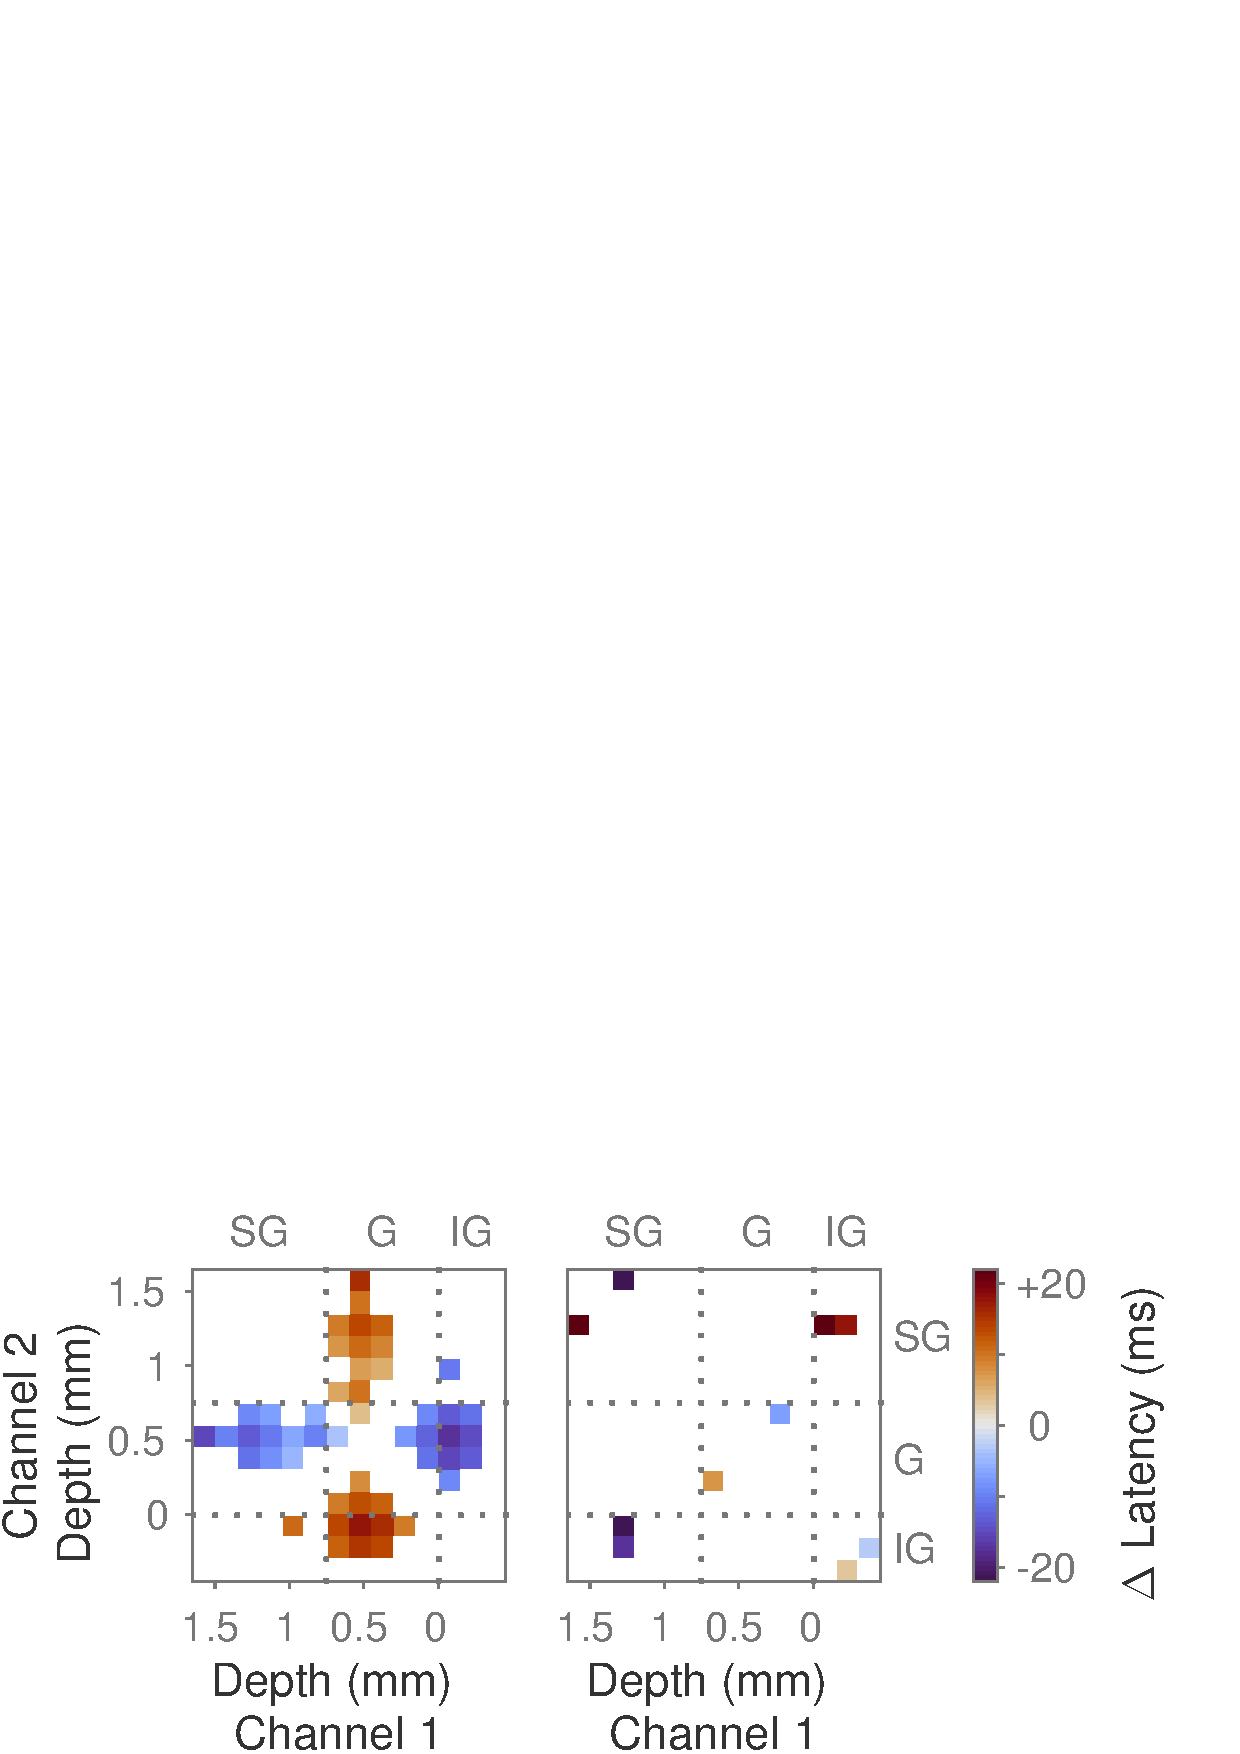
\includegraphics[scale=.5]{lag/latencydifference-avg.png}
    \caption{
Difference in peak information latency for each pair of channels in the cortical depth, computed from Channel 1 to Channel 2 (if $\Delta$ is positive, Channel 1 leads).
Left: latency for peak information in the power of \SIrange{4}{16}{Hz} oscillations about luminance changes at scale \SI{<0.3}{cpd}.
Right: \SIrange{60}{170}{Hz} power about \SI{>1.0}{cpd}.
Mean of 6 sessions.
Pairs of channels with no significant difference between their information latency (Student's t-test) are indicated in white.
}
\label{fig:lam_lag_dif}
\end{figure}


%-------------------------------------------------------------------------------
\section{Discussion}
%-------------------------------------------------------------------------------
